\documentclass[9pt]{acm_proc_article-sp}
\usepackage{graphicx}
\usepackage{amsmath}
\usepackage{enumerate}
\usepackage{multirow}
\usepackage{epstopdf}
\usepackage{array}
\usepackage{CJK}
\usepackage{float}
\usepackage{subfigure}
\usepackage{algorithm}
\usepackage{algorithmicx}
\newcommand{\algorithmicbreak}{\textbf{break}}
\newcommand{\BREAK}{\State \algorithmicbreak}
\usepackage{algpseudocode}
\begin{document}

\title{A Sample {\ttlit ACM} SIG Proceedings Paper in LaTeX Format}

\numberofauthors{1}
\author{
% 1st. author
\alignauthor
Zhen Chen, Huizhen Jiang, Haifeng Liu\\
       \affaddr{School of Software, Dalian University of Technology, Dalian 116620, China.}\\
       \email{f.xia@acm.org}
%% 2nd. author
%\alignauthor
%G.K.M. Tobin\titlenote{The secretary disavows
%any knowledge of this author's actions.}\\
%       \affaddr{Institute for Clarity in Documentation}\\
%       \affaddr{P.O. Box 1212}\\
%       \affaddr{Dublin, Ohio 43017-6221}\\
%       \email{webmaster@marysville-ohio.com}
%% 3rd. author
%\alignauthor Lars Th{\o}rv{\"a}ld\titlenote{This author is the
%one who did all the really hard work.}\\
%       \affaddr{The Th{\o}rv{\"a}ld Group}\\
%       \affaddr{1 Th{\o}rv{\"a}ld Circle}\\
%       \affaddr{Hekla, Iceland}\\
%       \email{larst@affiliation.org}
%\and  % use '\and' if you need 'another row' of author names
%% 4th. author
%\alignauthor Lawrence P. Leipuner\\
%       \affaddr{Brookhaven Laboratories}\\
%       \affaddr{Brookhaven National Lab}\\
%       \affaddr{P.O. Box 5000}\\
%       \email{lleipuner@researchlabs.org}
%% 5th. author
%\alignauthor Sean Fogarty\\
%       \affaddr{NASA Ames Research Center}\\
%       \affaddr{Moffett Field}\\
%       \affaddr{California 94035}\\
%       \email{fogartys@amesres.org}
%% 6th. author
%\alignauthor Charles Palmer\\
%       \affaddr{Palmer Research Laboratories}\\
%       \affaddr{8600 Datapoint Drive}\\
%       \affaddr{San Antonio, Texas 78229}\\
%       \email{cpalmer@prl.com}
}
% There's nothing stopping you putting the seventh, eighth, etc.
% author on the opening page (as the 'third row') but we ask,
% for aesthetic reasons that you place these 'additional authors'
% in the \additional authors block, viz.
%\additionalauthors{Additional authors: John Smith (The Th{\o}rv{\"a}ld Group,
%email: {\texttt{jsmith@affiliation.org}}) and Julius P.~Kumquat
%(The Kumquat Consortium, email: {\texttt{jpkumquat@consortium.net}}).}
%\date{30 July 1999}
% Just remember to make sure that the TOTAL number of authors
% is the number that will appear on the first page PLUS the
% number that will appear in the \additionalauthors section.

\maketitle
\begin{abstract}

\end{abstract}

% A category with the (minimum) three required fields
\category{H.4}{Information Systems Applications}{Miscellaneous}
%A category including the fourth, optional field follows...
\category{D.2.8}{Software Engineering}{Metrics}[complexity measures, performance measures]

\terms{Theory}

\keywords{ACM proceedings, \LaTeX, text tagging}

\section{Introduction}

\section{Related work}

%\begin{table}
%\centering
%\caption{Frequency of Special Characters}
%\begin{tabular}{|c|c|l|} \hline
%Non-English or Math&Frequency&Comments\\ \hline
%\O & 1 in 1,000& For Swedish names\\ \hline
%$\pi$ & 1 in 5& Common in math\\ \hline
%\$ & 4 in 5 & Used in business\\ \hline
%$\Psi^2_1$ & 1 in 40,000& Unexplained usage\\
%\hline\end{tabular}
%\end{table}


%\begin{table*}
%\centering
%\caption{Some Typical Commands}
%\begin{tabular}{|c|c|l|} \hline
%Command&A Number&Comments\\ \hline
%\texttt{{\char'134}alignauthor} & 100& Author alignment\\ \hline
%\texttt{{\char'134}numberofauthors}& 200& Author enumeration\\ \hline
%\texttt{{\char'134}table}& 300 & For tables\\ \hline
%\texttt{{\char'134}table*}& 400& For wider tables\\ \hline\end{tabular}
%\end{table*}
% end the environment with {table*}, NOTE not {table}!

\begin{figure}
\centering
\includegraphics [width=3.5in]{Fig1.pdf}
\caption{A sample black and white graphic (.eps format).}
\end{figure}
\begin{figure}
\centering
\includegraphics [width=2.5in]{Fig2.pdf}
\caption{A sample black and white graphic (.eps format).}
\end{figure}

\begin{figure}
\centering
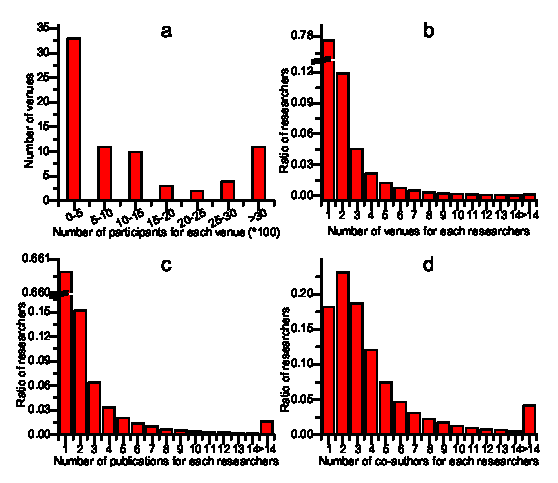
\includegraphics [width=3.5in]{Fig3.eps}
\caption{A sample black and white graphic (.eps format).}
\end{figure}
\begin{figure*}
\centering
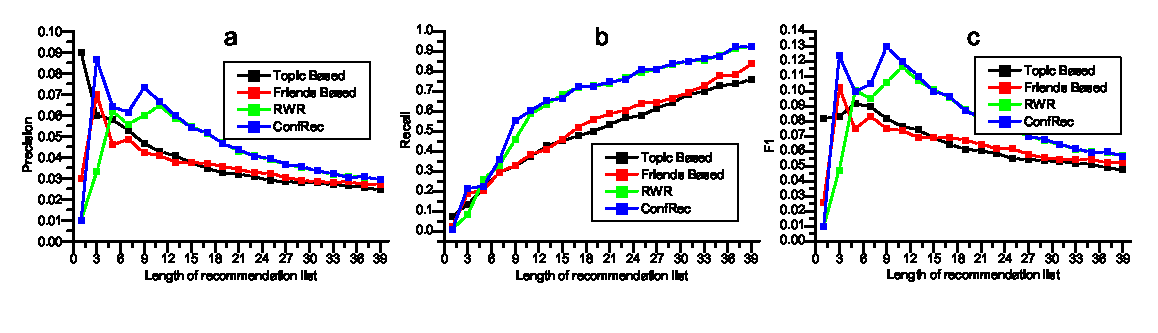
\includegraphics [width=\textwidth]{Fig4.eps}
\caption{A sample black and white graphic (.eps format).}
\end{figure*}
\begin{figure*}
\centering
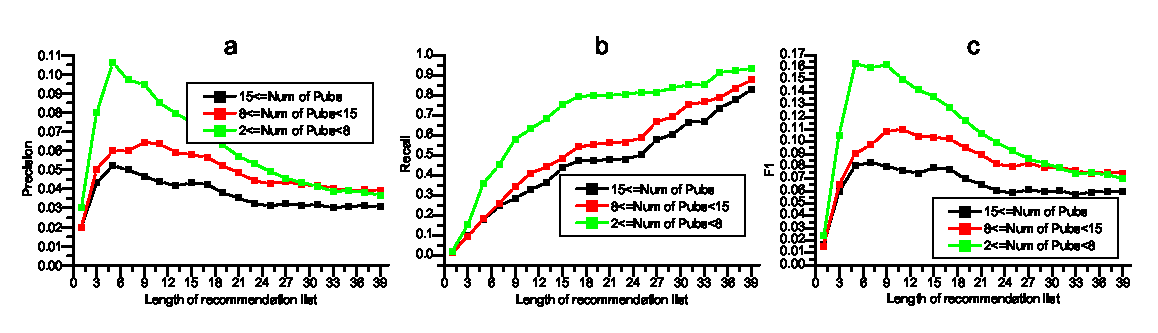
\includegraphics [width=\textwidth]{Fig5.eps}
\caption{A sample black and white graphic (.eps format).}
\end{figure*}
%
%\begin{figure}
%\centering
%\epsfig{file=fly.eps, height=1in, width=1in}
%\caption{A sample black and white graphic (.eps format)
%that has been resized with the \texttt{epsfig} command.}
%\end{figure}

%
%\begin{figure}
%\centering
%\psfig{file=rosette.ps, height=1in, width=1in,}
%\caption{A sample black and white graphic (.ps format) that has
%been resized with the \texttt{psfig} command.}
%\end{figure}

%\begin{figure*}
%\centering
%\epsfig{file=flies.eps}
%\caption{A sample black and white graphic (.eps format)
%that needs to span two columns of text.}
%\end{figure*}

\section{Conclusions}

%\end{document}  % This is where a 'short' article might terminate

%ACKNOWLEDGMENTS are optional
\section{Acknowledgments}

\bibliographystyle{abbrv}
\bibliography{ConfRec}
\appendix
%Appendix A
\balancecolumns
\end{document}
